\chapter{Prezentacja działania}
W nieniejszym rozdziale przedstawiono działanie systemu. Opisano w nim poszczególne ekrany aplikacji oraz ich funkcjonalność. 

\section{Ekran startowy}
Po uruchomieniu aplikacji, pierwszym ekranem widocznym dla użytkownika, jest ekran startowy, przedstawiony na rysunku \ref{fig:homescreen}. Składa się on z czterach przycisków, które po naciśnięciu przekierowują użytkownika do odpowiednich sekcji aplikacji.

 \begin{figure}[h]
     \centering
     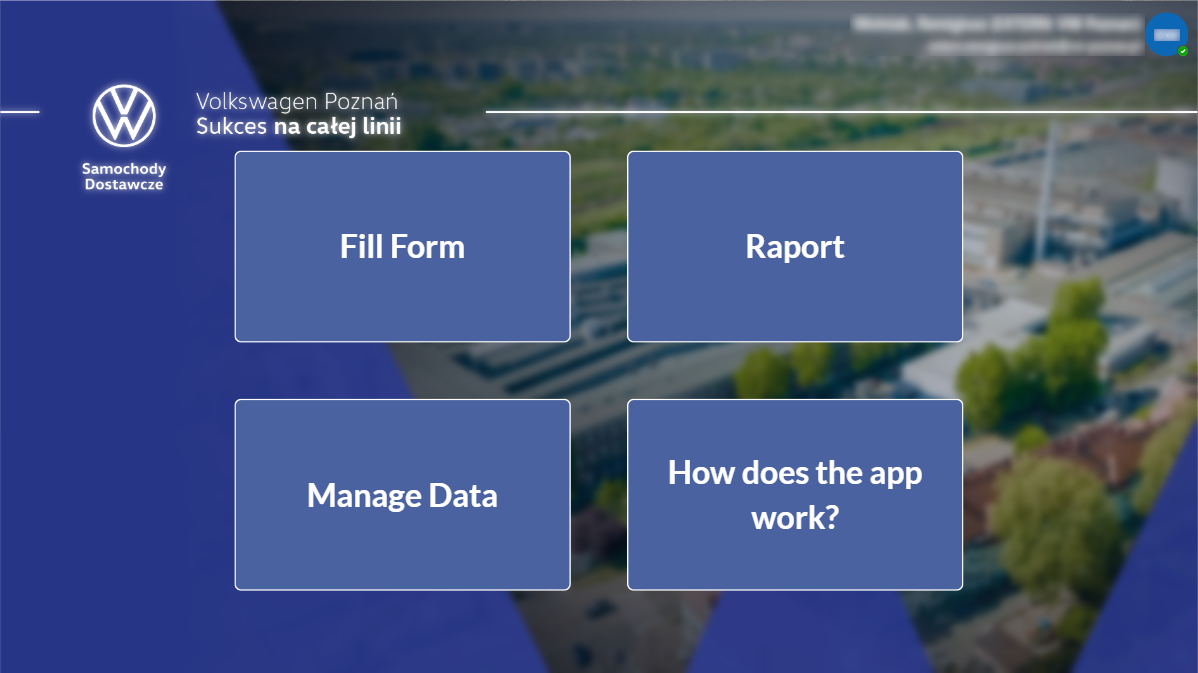
\includegraphics[width=0.9\textwidth]{figures/HomeScreen.png}
     \caption{Ekran startowy aplikacji} 
     \label{fig:homescreen}
 \end{figure}

 Ten ekran aplikacji, pełni funkcję panelu nawigacji dla użytkownika, umożliwiając intuicyjne poruszanie się po innych sekcjach systemu.
Poniżej przedstawiono, który przycisk odpowiada za przekierowanie do danej sekcji aplikacji:
\begin{itemize}
    \item \emph{Manage Data} $\rightarrow$ Ekran dodawania danych,
    \item \emph{Fill Form} $\rightarrow$ Ekran wypełniania formularza,
    \item \emph{Raport} $\rightarrow$ Ekran generowania raportu,
    \item \emph{How does tha app work?} $\rightarrow$ Ekran samouczka.
\end{itemize}


 \section{Ekran dodawania danych}
 Rysunek \ref{fig:managedatascreen} przedstawia ekran dodawania danych do systemu. Przeznaczony jest on do wprowadzenia nowych informacji o serwisach, które pochodzą z arkusza kalkulacyjnego.
  \begin{figure}[H]
     \centering
     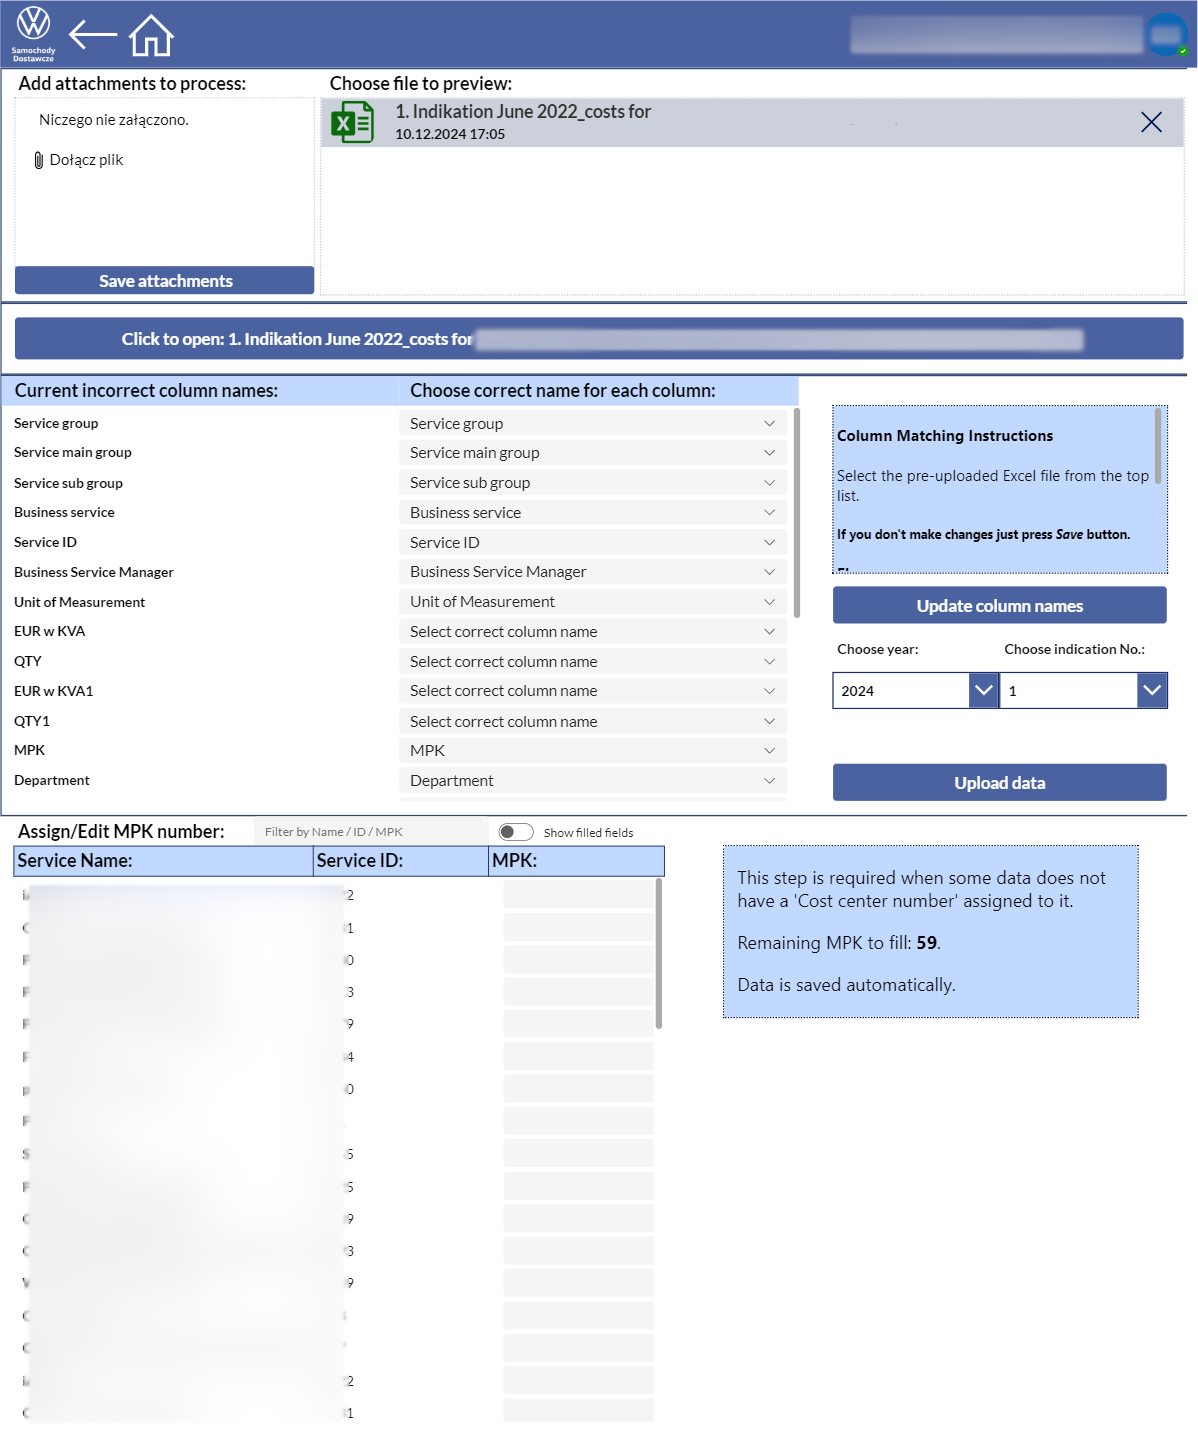
\includegraphics[width=0.9\textwidth]{figures/ManageDataScreen.png}
     \caption{Ekran dodawania danych do systemu} 
     \label{fig:managedatascreen}
 \end{figure}

 Ekran ten podzielony został na trzy główne sekcje:
 \begin{itemize}
    \item Sekcja dodawania pliku do systemu,
    \item Formularz walidacji kolumn,
    \item Formularz uzupełniania numerów MPK.
 \end{itemize}

 \subsection*{Sekcja dodawania pliku do systemu}
 \begin{figure}[H]
     \centering
     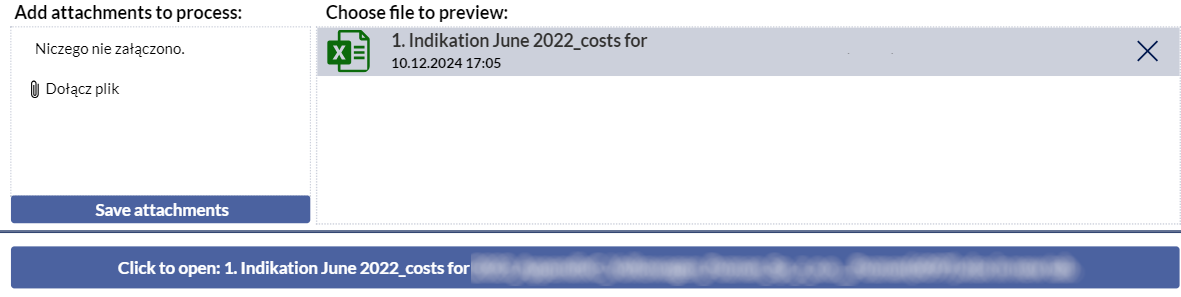
\includegraphics[width=\textwidth]{figures/SaveAttachmentsForm.png}
     \caption{Formularz zapisu plików do systemu}
     \label{fig:SaveAttachmentsForm}
 \end{figure}
 Rysunek \ref{fig:SaveAttachmentsForm} zawiera elementy służące do dodawaniu plików do systemu oraz nawigacji po nich.

 Kontrolka opisana jako \emph{Add attachments to process}, pozwala na dodanie nowego arkusza kalkulacyjnego do systemu. Wybór pliku odbywa się przy pomocy przycisku \emph{Add attachments} lub z użyciem mechaniki \emph{Drag\&Drop}. Kiedy plik zostanie pomyślnie dodany do pamięci aplikacji, wyświetli się on na liście.

 Aby plik został dodany do bilbioteki SharePoint, należy nacisnąć przycisk \emph{Save attachments} znajdujący się podniżej. Naciśnięcie przycisku skutkuje rozpoczęciem procesu zapisu oraz wstępnego formatowania danych. W tym czasie na ekranie widoczny będzie wskaźnik informujący użytkownika o trwającym procesie.

 Po prawej stronie znajduje się lista plików, które zostały poprawnie zapisane w folderze tymczasowym Sharepoint. Lista ta pozwala na wybór pliku, który zostanie przetworzony w kolejnych krokach. Dodatkowo krzyżyk przy każdym pliku pozwala na usunięcie go z systemu -- w tym z folderu tymczasowego.
 
 Ostatnim elementem tej sekcji jest przycisk \emph{Clock to open:...}.
 Jego naciśnięcie skutkuje otwarciem pliku wybranego z listy w nowej karcie przeglądarki. Pozwala to na weryfikację poprawności zapisanego pliku oraz jest pomocne w kolejnym kroku procesu.

\subsection{Formularz walidacji kolumn} 
  \begin{figure}[h]
     \centering
     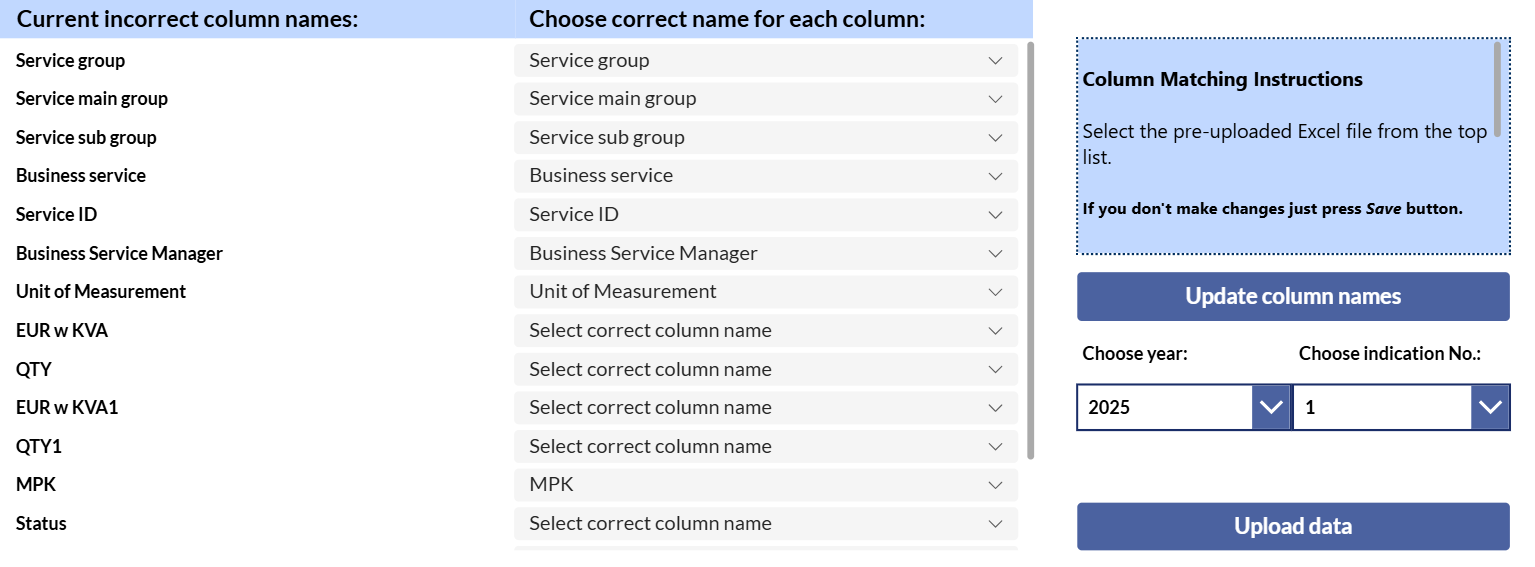
\includegraphics[width=\textwidth]{figures/ColumnMappingForm.png}
     \caption{Formularz walidacji nazw kolumn}
     \label{fig:columnmappingform}
 \end{figure}

Głównym elementem formularza jest dwukolumnowa galeria, dzięki której użytkownik może dostosować nazwy kolumn w arkuszu kalkulacyjnym do nazw kolumn w bazie danych. W lewej kolumnie znajdują się nagłówki pobrane z arkusza natomiast w prawej kolumnie znajdują się rozwijane listy pozwalające na dopasowanie odpowiedniej nazwy. Na rysunek \ref{fig:columnmappingform} widać, że niektóre nazwy zostały już przypisane. Wynika to z działania skryptu, który automatycznie podpowiada ich nazwę co pozwala przyspieszyć ten krok. Tutaj również przydatna jest funkcja podglądu pliku, ponieważ pozwala ona na określenie prawidłowej nazwy na podstawie zawartości kolumny.

Po prawej stronie umieszczono dodatkowe kontrolki. Pierwszą z nich, jest krótka instrukcja dla użytkownika, umieszczona na niebieskim tle.
Pod nią znajduje sie przycisk \emph{Update column names}, który pozwala na zapisanie zmian w nazwach kolumn. Po jego naciśnięciu, wyświetlone zostanie okno dialogowe (rysunek \ref{fig:CorrectHeadersPopup}) z zapytaniem o potwierdzenie zmian. Zmiana nazw kolumn jest bardzo ważny dla dalszego działania aplikacji, dlatego zaleca się dokładne sprawdzenie poprawności wybranych nazw.
\begin{figure}[h]
    \centering
    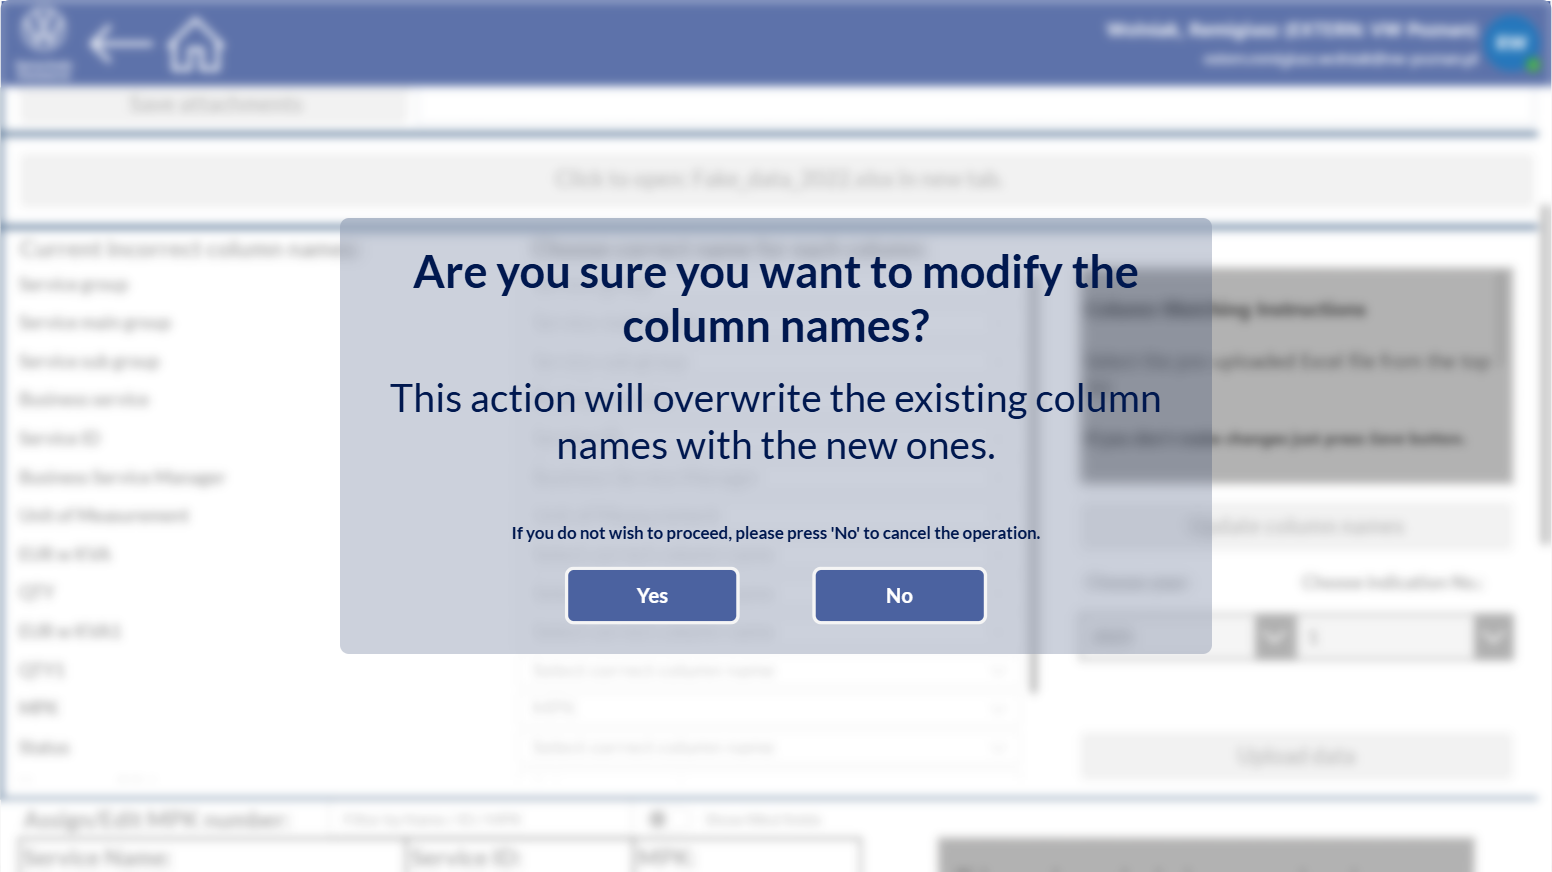
\includegraphics[width=\linewidth]{figures/CorrectHeadersPopup.png}
    \caption{Zapytanie o poprawność nazw kolumn}
    \label{fig:CorrectHeadersPopup}
\end{figure}
Zatwierdzenie zmiany, skutkuje rozpoczęciem procesu nadpisania nagłówków, oczym informuje odpowiedni indykator. Po zakończeniu procesu, galeria z nazwami kolumn zostaje zaaktualizowana.

Formularz ten pozwala również na przesłanie danych z arkusza do bazy danych. Pierwszym krokiem jest wybór roku oraz numeru indykacji, których dotyczą dane przy użyciu rozwijanych list znajdujących się pod przyciskiem aktualizującym nazwy kolumn. Kiedy wybrano odpowiednie wartości, można zainicjować proces zapisu danych poprzez użycie przycisku \emph{Upload data}. Naciśnięcie go skutkuje trzema scenariuszami:
\begin{itemize}
    \item Kiedy nie zmieniono nazw kolumn, wyświetlone zostaje okno dialogowe z rysunku \ref{fig:columnmappingform}. Ma to na celu upewnienie się, że nagłówki są poprawne.
    \item Kiedy wybrano rok i numer indykacji dla których informacje istnieją już w bazie danych, wyświetlone zostaje okno dialogowe widoczne na rysunku \ref{fig:DoYouWantToOverwrite}. Informuje ono użytkownika, o istniejących danych i daje możliwość ich nadpisania lub anulowania operacji.
    \item Kiedy nazwy zostału uprzednio zmienione i kiedy wybrano unikalne wartości dla roku i numeru indykacji, proces zapisu danych zostaje rozpoczęty bez dodatkowych zapytań.
\end{itemize}

Występuje również przypadek kiedy omówione okna dialogowe wyświetlają się jedno o drugim. W takiej sytuacji, użytkownik musi najpierw potwierdzić zmianę nazw kolumn, a następnie zdecydować czy chce nadpisać dane.

\begin{figure}[h]
            \centering
            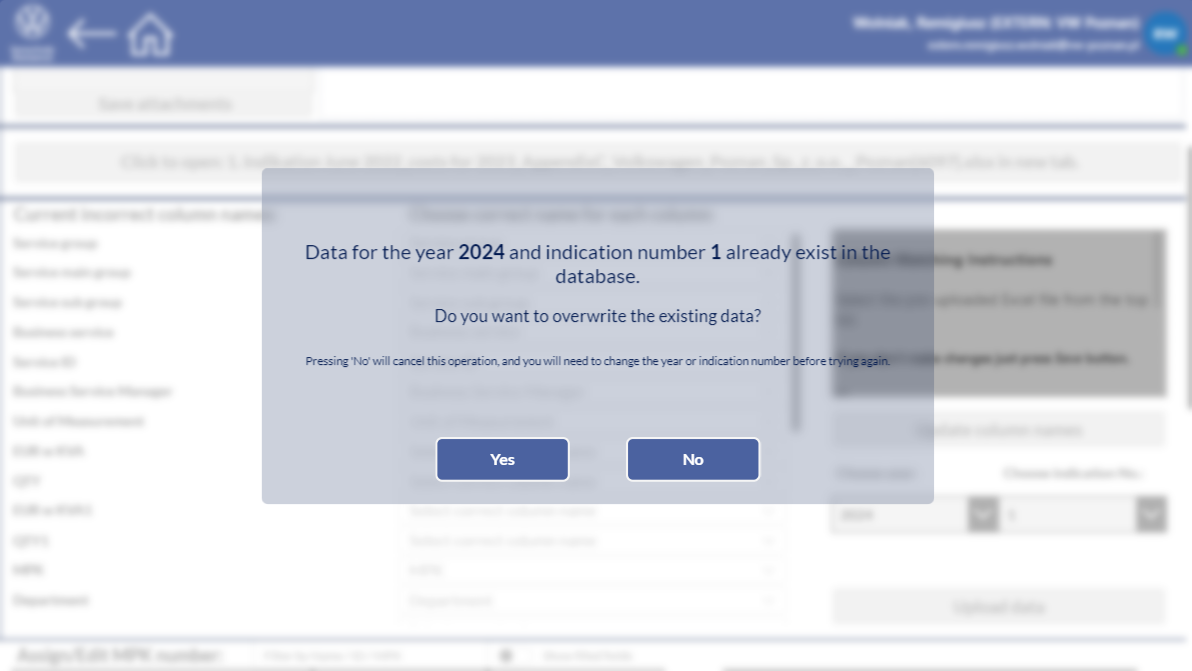
\includegraphics[width=\linewidth]{figures/DoUWantToOverwrite.png}
            \caption{Zapytanie o nadpisanie danych}
            \label{fig:DoYouWantToOverwrite}
        \end{figure}

Proces zapisu danych jest najdłużej trwającym etapem. Czas zapisu wynosi od 30 do 60 sekund w zależności od ilości danych oraz jakości połączenia z serwerem. Z uwagi na wykorzystanie mechanizmu zapisu z użyciem żądań zbiorowychm, nie jest możliwe poinformowanie użytkownika o postępie operacji.

Po ukończeniu operacji wyświetlana jest informacja o zakończeniu procesu. Użytkownik zostanie również poinformowany w razie wystąpienia błędów.

\subsection{Formularz uzupełniania numerów MPK}
 \begin{figure}[h]
     \centering
     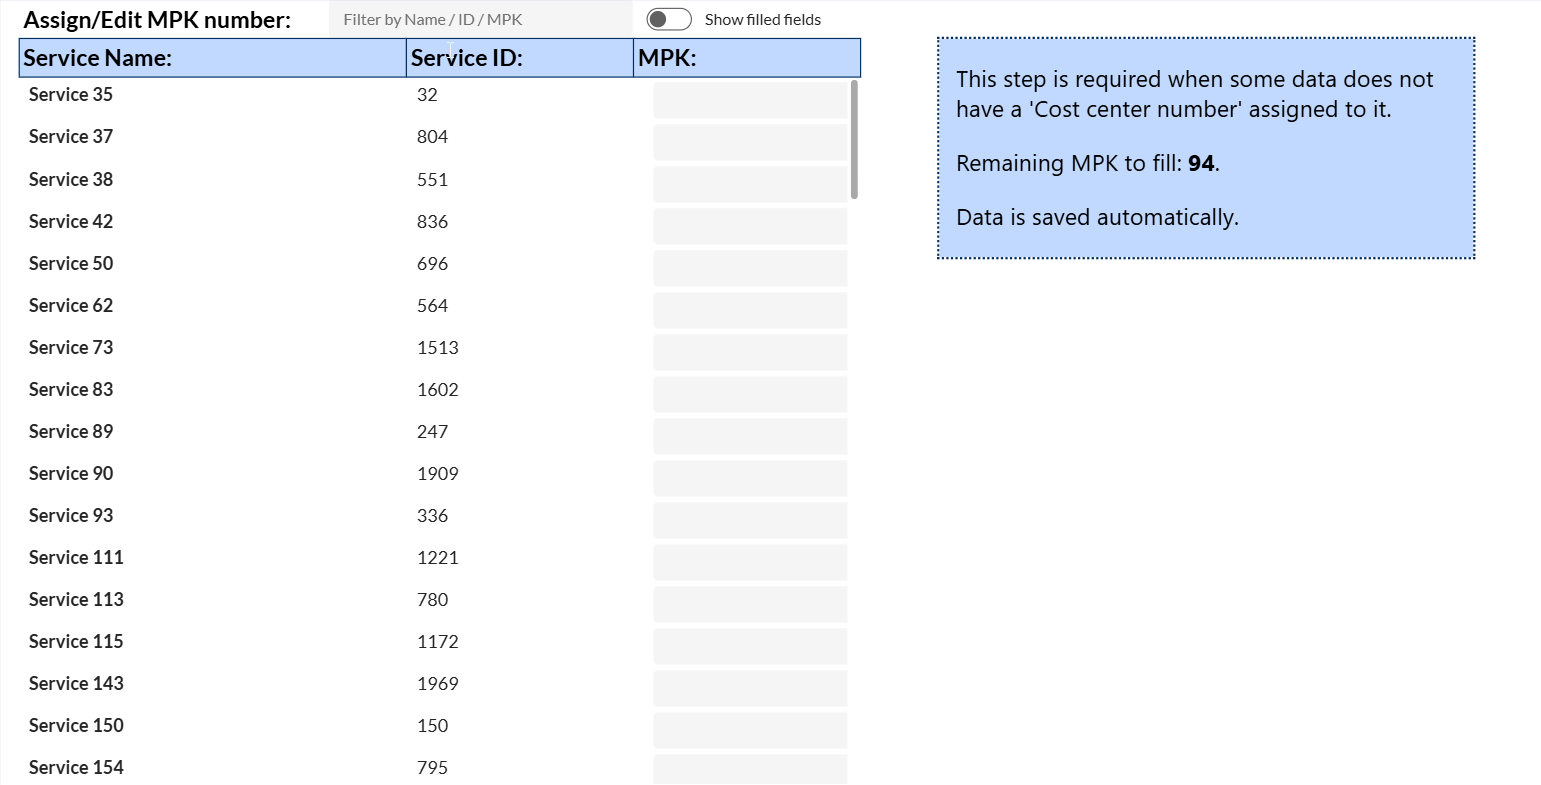
\includegraphics[width=\textwidth]{figures/FillMPKForm.png}
     \caption{Formularz wypełniania/edycji numerów MPK}
     \label{fig:fillmpkform}
 \end{figure}

 Ostatnią sekcją tego ekranu jst formularz edycji numerów MPK widoczny na rysunku \ref{fig:fillmpkform}. 

 Składa się on z galerii zawierającej następujące kolumny:
 \begin{itemize}
    \item \emph{Service Name} -- nazwa serwisu,
    \item \emph{Service ID} -- unikalny identyfikator serwisu,
    \item \emph{MPK} -- miejsce powstawania kosztów.
 \end{itemize}
 Ostatnia z nich jest edytowalna, co pozwala na nadanie lub zmianę numeru MPK. Zmiany są automatyczie zapisywane.

 Nad galerią umieszczono pole tekstowe, które pozwala na filtrowanie wyników względem każdej z kolumn. \\Obok znajduje się przełącznik, kótry pozwala na przełączenie się miedzy widokiem wypełnionych oraz pustych numerów MPK.\\
 Należy pamiętać, że system automatycznie przypisuje numer MPK na podstawie informacji z poprzedniego roku co pozwala na minimalizację wprowadzanych danych.

 Po  prawej stronie znajduje się kolejne pole informacyjne, które zawiera instrukcję dla użytkownika oraz liczbę serwisów, które nie są przypisane do żadnego obszaru.
\vspace{0.5cm}

Taki układ formularza pozwala na szybkie dodanie danych do systemu pozwalając na elastyczne dostosowanie ich do struktury bazy danych.

\section{Ekran wypełniania formularza}
Proces podejmowania decyzji odbywa się osobno dla każdej z usług. Dlatego ta część aplikacji składa się z dwóch ekranów: ekranu nawigacyjnego oraz ekranu szczegółowego.

\subsection{Ekran nawigacyjny}
 \begin{figure}[h]
 \centering
 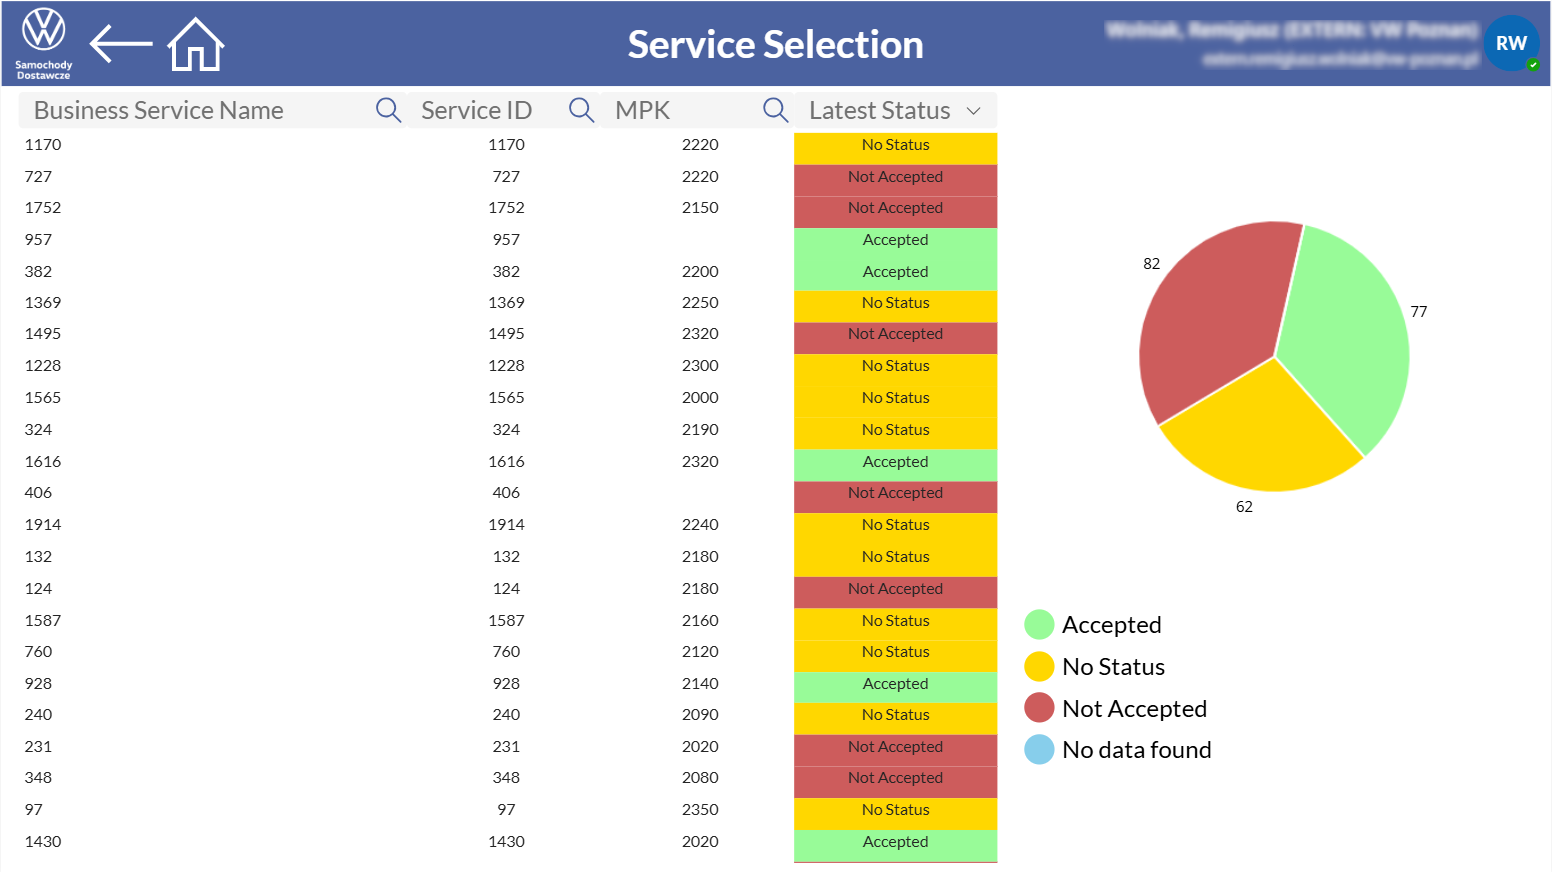
\includegraphics[width=0.9\textwidth]{figures/ServiceSelectionForm.png}
 \caption{Ekran wyboru usługi do edycji}
 \label{fig:ServiceSelectionForm }
 \end{figure}

 Na tym ekranie umieszczono listę wszystkich serwisów, które znajdują się w bazie danych. Użytkownik ma możliwość filtrowania oraz wyszukiwania serwisów według różnych kryteriów poprzez pola znajdujące sę nad listą.

 Po naciśnięciu wiersza odpowiadającego serwisowi, użytkownik zostaje przekierowany do ekranu szczegółowego.

 Dodatkowo, po prawej stronie znajduje się wykres kołowy. Każdy segment odpowiada liczbie elementów z przypisanym statusem, co pozwala użytkownikowi szybko ocenić proporcje między kategoriami (\emph{Accepted}, \emph{Not Accepted}, \emph{No Status}). Wykres jest dynamiczny — aktualizuje się w czasie rzeczywistym w oparciu o zastosowane filtry, co zapewnia aktualność prezentowanych informacji.